%%%%%%%%%%%%%%%%%%%%%%%%%%%%%%%%%%%%%
%                                   %
% Compile with XeLaTeX and biber    %
%                                   %
% Questions or comments:            %
%                                   %
% joshua dot mcneill at uga dot edu %
%                                   %
%%%%%%%%%%%%%%%%%%%%%%%%%%%%%%%%%%%%%

\documentclass{beamer}
  % Read in standard preamble (cosmetic stuff)
  %%%%%%%%%%%%%%%%%%%%%%%%%%%%%%%%%%%%%%%%%%%%%%%%%%%%%%%%%%%%%%%%
% This is a standard preamble used in for all slide documents. %
% It basically contains cosmetic settings.                     %
%                                                              %
% Joshua McNeill                                               %
% joshua dot mcneill at uga dot edu                            %
%%%%%%%%%%%%%%%%%%%%%%%%%%%%%%%%%%%%%%%%%%%%%%%%%%%%%%%%%%%%%%%%

% Beamer settings
% \usetheme{Berkeley}
\usetheme{CambridgeUS}
% \usecolortheme{dove}
% \usecolortheme{rose}
\usecolortheme{seagull}
\usefonttheme{professionalfonts}
\usefonttheme{serif}
\setbeamertemplate{bibliography item}{}

% Packages and settings
\usepackage{fontspec}
  \setmainfont{Charis SIL}
\usepackage{hyperref}
  \hypersetup{colorlinks=true,
              allcolors=blue}
\usepackage{graphicx}
  \graphicspath{{../../figures/}}
\usepackage[normalem]{ulem}
\usepackage{enumerate}

% Document information
\author{M. McNeill}
\title[FREN2001]{Français 2001}
\institute{\url{joshua.mcneill@uga.edu}}
\date{}

%% Custom commands
% Lexical items
\newcommand{\lexi}[1]{\textit{#1}}
% Gloss
\newcommand{\gloss}[1]{`#1'}
\newcommand{\tinygloss}[1]{{\tiny`#1'}}
% Orthographic representations
\newcommand{\orth}[1]{$\langle$#1$\rangle$}
% Utterances (pragmatics)
\newcommand{\uttr}[1]{`#1'}
% Sentences (pragmatics)
\newcommand{\sent}[1]{\textit{#1}}
% Base dir for definitions
\newcommand{\defs}{../definitions}


  % Document information
  \subtitle[Intro to Semantics]{Introduction to Semantics}

  %% Custom commands
  % Subsection/frame titles
  \newcommand{\suboneone}{What is it?}
  \newcommand{\subonetwo}{What do we mean by meaning?}
  \newcommand{\subtwoone}{}

\begin{document}
  % Read in the standard intro slides (title page and table of contents)
  %%%%%%%%%%%%%%%%%%%%%%%%%%%%%%%%%%%%%%%%%%%%%%%%%%%%%%%%%%%%%%%%
% This is a standard set of intro slides used in for all slide %
% documents. It basically contains the title page and table of %
% contents.                                                    %
%                                                              %
% Joshua McNeill                                               %
% joshua dot mcneill at uga dot edu                            %
%%%%%%%%%%%%%%%%%%%%%%%%%%%%%%%%%%%%%%%%%%%%%%%%%%%%%%%%%%%%%%%%

\begin{frame}
  \titlepage
  \tiny{Office: % Basically a variable for office hours location
Gilbert 121\\
        Office hours: % Basically a variable for office hours
 lundi, mercredi, vendredi 10:10--11:10
}
\end{frame}

\begin{frame}
  \tableofcontents[hideallsubsections]
\end{frame}

\AtBeginSection[]{
  \begin{frame}
    \tableofcontents[currentsection,
                     hideallsubsections]
  \end{frame}
}


  \section{Semantics Basics}
    \subsection{\suboneone}
      \begin{frame}{\suboneone}
        \begin{definition}
          % Semantics
The study of meaning

        \end{definition}
        \begin{example}<2->
          We said that \lexi{bank}\textsubscript{1} and \lexi{bank}\textsubscript{2} have unrelated meanings:
          \begin{itemize}
            \item How does that work?
            \item How do we model that?
          \end{itemize}
        \end{example}
      \end{frame}

      \begin{frame}{\suboneone}
        \begin{block}{Two broad areas of semantics}
          \begin{itemize}
            \item Lexical semantics
            \item Compositional semantics
          \end{itemize}
        \end{block}
        \begin{alertblock}{Lexical semantics}
          % Lexical semantics
The area of semantics concerned with the meanings of lexical expressions

        \end{alertblock}
        \begin{alertblock}{Compositional semantics}
          % Compositional semantics
The area of semantics concerned with the meanings created through the combination of multiple lexical expressions

        \end{alertblock}
      \end{frame}

    \subsection{\subonetwo}
      \begin{frame}[t]{\subonetwo}
        \begin{block}{Two aspects of meaning}
          \begin{itemize}
            \item \alert{Sense}: % Sense
A meaning of a linguistic expression in terms of its relationship with the rest of the language of which it is part

            \item \alert{Reference}: % Reference
The connection between a linguistic expression and an object in the world

          \end{itemize}
        \end{block}
        \only<2>{
          \begin{example}
            The senses of \lexi{dog}:
            \begin{itemize}
              \item \lexi{pet}, \lexi{furry}, \lexi{four legs}, \lexi{mammal}, \lexi{companion}, \lexi{canine}, etc.
            \end{itemize}
          \end{example}
        }
        \only<3-4>{
          \begin{example}
            \parbox{0.48\linewidth}{
              The reference for \lexi{dog}:
              \begin{itemize}
                \item<4-> \alert{Referent}: % Referent
The thing in the world to which a linguistic expression is connected

              \end{itemize}
            }
            \parbox{0.48\linewidth}{
              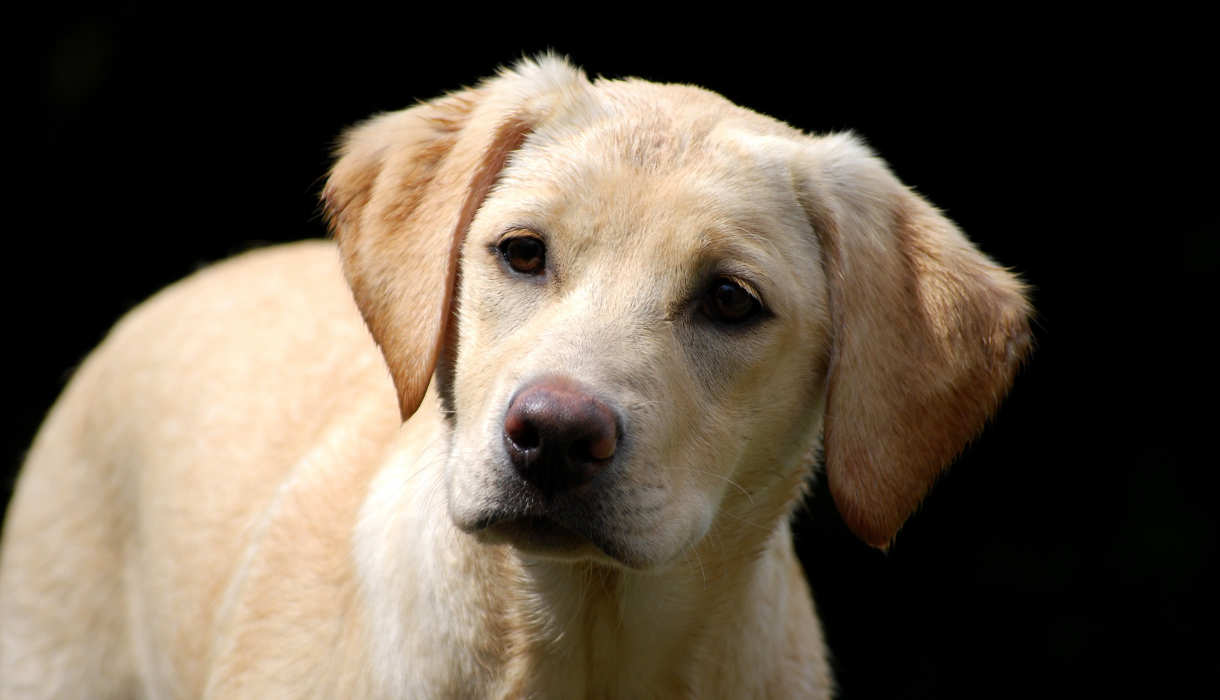
\includegraphics[scale=0.48]{dog.jpg}
            }
          \end{example}
        }
      \end{frame}

      % \begin{frame}{\subonetwo}
      %   \begin{block}{}
      %     \begin{itemize}
      %       \item Identifying the referent of an expression requires knowing its sense(s), but
      %       \item Knowing its senses does not mean you can pick out its referent
      %     \end{itemize}
      %   \end{block}
      %   \begin{example}
      %     \parbox{0.48\linewidth}{
      %       Is this a diamond?
      %       \begin{itemize}
      %         \item<2-> Cubic zirconia
      %       \end{itemize}
      %     }
      %     \parbox{0.48\linewidth}{
      %       \includegraphics[scale=0.35]{cubic_zirconia.jpg}
      %     }
      %   \end{example}
      % \end{frame}

      % Things probably not to cover
        % They claim that unicorn has no reference, just senses
        % They claim the same for Queen of the US

      \begin{frame}{\subonetwo}
        \begin{center}
          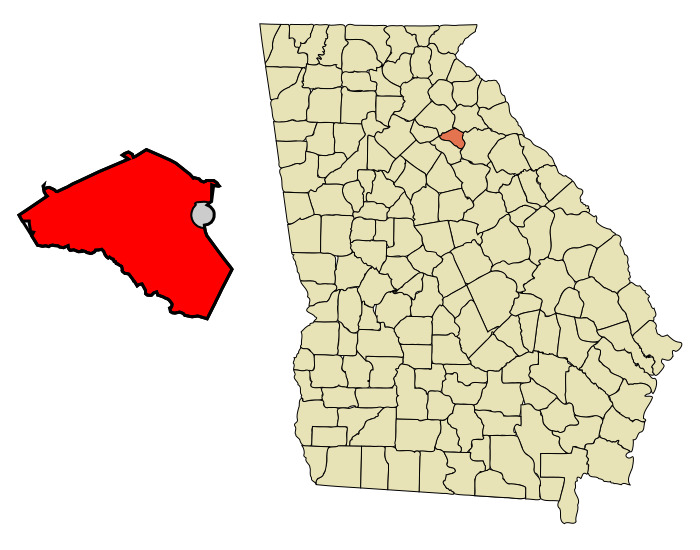
\includegraphics[scale=0.17]{athens.jpg}
        \end{center}
        \begin{columns}
          \column{0.5\linewidth}
            \begin{block}{\lexi{the city where R.E.M. got their start}}
              Senses:
              \begin{itemize}
                \item \lexi{Athens}, \lexi{Georgia}, \lexi{music}, \lexi{alternative}, etc.
              \end{itemize}
            \end{block}
          \column{0.5\linewidth}
            \begin{block}{\lexi{the city where UGA is located}}
              Senses:
              \begin{itemize}
                \item \lexi{Athens}, \lexi{Georgia}, \lexi{university}, etc.
              \end{itemize}
            \end{block}
        \end{columns}
      \end{frame}

  \section{Lexical Semantics}
    \subsection{\subtwoone}
      \begin{frame}{\subtwoone}

      \end{frame}

\end{document}
